\paragraph{QuizziPedia::Front-End::Directives::UserResultsDirective}

\label{QuizziPedia::Front-End::Directives::UserResultsDirective}

\begin{figure}[h]
	\centering
	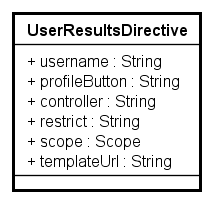
\includegraphics[scale=0.80,keepaspectratio]{UML/Classi/Front-End/QuizziPedia_Front-end_Directives_UserResultsDirective.png}
	\caption{QuizziPedia::Front-End::Directives::UserResultsDirective}
\end{figure}

\begin{itemize}
	\item \textbf{Descrizione}: directive che permette di visualizzare la lista degli utenti ricercati dopo aver utilizzato l'apposita funzione di ricerca;
	\item \textbf{Utilizzo}: permette di visualizzare la lista degli utenti, in particolare conterrà:
	\begin{itemize}
		\item Username dell'utente;
		\item Pulsante per poter essere reindirizzati alla pagina di visualizzazione del profilo dell'utente selezionato.
	\end{itemize}
	\item \textbf{Relazioni con altre classi}:
	\begin{itemize}
		\item \textbf{IN \texttt{ResultsModelView}}: classe di tipo modelview la cui istanziazione è contenuta all'interno della variabile di ambiente \$scope di \textit{Angular\ped{G}}. All'interno di essa sono presenti le variabili e i metodi necessari per il \textit{Two-Way Data-Binding\ped{G}} tra la view \texttt{ResultsView}, le directive e il \textit{controller\ped{G}} \texttt{SearchController};
		\item \textbf{OUT \texttt{ResultsView}}: view contenente i risultati della ricerca effettuata. Vengono visualizzati sia gli utenti che i questionari trovati;
		\item \textbf{IN \texttt{LangModel}}: rappresenta il modello delle informazioni per la giusta traduzione dell'applicazione.
	\end{itemize}
	\item \textbf{Attributi}:
	\begin{itemize}
		\item \texttt{+ username: String} \\ Attributo che conterrà l'username dell'utente;
		\item \texttt{+ profileButton: String} \\ Attributo che viene utilizzato per visualizzare la giusta traduzione della \textit{label\ped{G}} per il bottone di visualizzazione del profilo utente, in italiano o in inglese;
		\item \texttt{+ controller: String} \\ Stringa contenente il nome del \textit{controller\ped{G}} della direttiva;
		\item \texttt{+ restrict: String} \\ Stringa che permette di definire le modalità di inserimento della direttiva all'interno della pagina;
		\item \texttt{+ scope: Scope} \\Oggetto \texttt{\$scope} interno della direttiva, contiene le funzionalità per gestire i dati presenti all'interno;
		\item \texttt{+ templateUrl: String} \\ Stringa contenente il percorso del file \textit{HTML\ped{G}} che contiene la direttive.
	\end{itemize}
\end{itemize}
